\documentclass[t, aspectratio=169]{beamer} % Khai báo tỉ lệ cho Beamer biết
\usepackage[utf8]{vietnam}
\usepackage{amsthm,amsmath,amssymb}
\usepackage{lmodern}
\usepackage{graphicx}
\usepackage{booktabs}

% --- CẤU HÌNH LỀ ---
\def\slideContentLeftMargin{0.5cm}
\def\slideContentRightMargin{1cm}
\def\hustHeaderHeight{1cm}
\def\slideContentBotMargin{3.5cm}

\usepackage[blue, 169]{beamerthemeHUST}

\renewcommand{\titlePageTitleX}{-0.5cm}
\renewcommand{\titlePageTitleY}{-0.5cm}
\renewcommand{\hustTitleAlign}{\alignLeft}
\renewcommand{\hustSubtitleAlign}{\alignLeft}
\renewcommand{\hustAuthorAlign}{\alignLeft}
\renewcommand{\hustInstAlign}{\alignLeft}

\title{ĐÁNH GIÁ MODULAR REPRESENTATION \& RECOGNIZER \\ TRONG NHẬN DIỆN BẢNG CHỮ ASL}
\subtitle{Computer Vision Capstone — Học kỳ 2025.2}
\author{\texorpdfstring{Trần Quang Hưng - 20235502 \\ Đỗ Đăng Vũ - 20235578 \\ Lê Hoàng Tùng - 20235572}{Trần Quang Hưng - 20235502, Đỗ Đăng Vũ - 20235578, Lê Hoàng Tùng - 20235572}}
\institute{Trường Công nghệ Thông tin và Truyền thông - ĐH Bách Khoa Hà Nội}

\begin{document}

	\hustintropage{}
	\hustsectionpage{}

	\husttitlepage

	\begin{frame}[allowframebreaks]{Nội dung trình bày}
		\tableofcontents
	\end{frame}

	\resetPageCount
	\showPageNumber

	\useStyleHustFull
	\useThinBar

	% =================================================================
	\section{Đặt vấn đề}
	% =================================================================
	\begin{frame}{1. Bối cảnh \& Động lực}
		\textbf{Bối cảnh thực tế:}
		\begin{itemize}
			\item Ngôn ngữ ký hiệu (ASL) là phương tiện giao tiếp chính của hàng triệu người khiếm thính.
			\item Hệ thống nhận diện ASL thời gian thực giúp giảm rào cản giao tiếp, không cần phần cứng chuyên dụng (chỉ cần webcam).
		\end{itemize}

		\vspace{1em}

		\textbf{Thách thức kỹ thuật:}
		\begin{itemize}
			\item Có rất nhiều lựa chọn kiến trúc: crop tay bằng detector hay dùng landmark? CNN hay Vision Transformer?
			\item \alert{Câu hỏi cốt lõi:} Một representation "thông minh hơn" (crop tay, trích landmark, tăng cường ảnh) có thực sự cải thiện nhận diện, hay chỉ thêm độ phức tạp và thêm điểm có thể gãy?
			\item Accuracy trên ảnh sạch có thể đánh lừa — cần đánh giá cả độ bền (robustness) dưới điều kiện thực tế.
		\end{itemize}
	\end{frame}

	% =================================================================
	\section{Mục tiêu \& Đóng góp}
	% =================================================================
	\begin{frame}{2. Mục tiêu \& Đóng góp}
		\begin{block}{Câu hỏi nghiên cứu}
			Liệu các representation tốt hơn (hand-crop, landmark, enhancement) có thực sự cải thiện nhận diện A--Z, hay chỉ thêm độ phức tạp mà không thêm giá trị?
		\end{block}

		\vspace{1em}

		\begin{columns}[T]
			\begin{column}{0.32\textwidth}
				\begin{block}{1. Framework module hóa}
					\small Tách riêng \textbf{Representation} và \textbf{Recognizer}, hoán đổi tự do — 13 pipeline khác nhau trên cùng 1 protocol.
				\end{block}
			\end{column}
			\begin{column}{0.32\textwidth}
				\begin{block}{2. Đánh giá đa chiều}
					\small Không chỉ accuracy sạch — còn macro-F1, robustness dưới 7--8 loại corruption, tỉ lệ phát hiện tay thất bại.
				\end{block}
			\end{column}
			\begin{column}{0.32\textwidth}
				\begin{block}{3. Phân tích trực quan sâu}
					\small Grad-CAM nội bộ CNN, UMAP/t-SNE không gian đặc trưng, qualitative grid so sánh từng bước pipeline.
				\end{block}
			\end{column}
		\end{columns}
	\end{frame}

	% =================================================================
	\section{Dữ liệu}
	% =================================================================
	\begin{frame}{3. Dataset Overview}
		\begin{table}
			\centering
			\small
			\begin{tabular}{lccc}
				\toprule
				\textbf{Tập dữ liệu} & \textbf{Vai trò} & \textbf{Số lớp} & \textbf{Quy mô} \\
				\midrule
				ASL Alphabet (Kaggle) train & Train classifier / landmark MLP & 26 (A--Z) & $\sim$78.000 ảnh \\
				ASL Alphabet test\_split & Đánh giá clean + robustness & 26 (A--Z) & 2.600 ảnh \\
				\bottomrule
			\end{tabular}
		\end{table}

		\vspace{1em}
		\textbf{Đặc điểm:} ảnh studio, nền tương đối sạch, ánh sáng đều $\Rightarrow$ \alert{dataset "dễ"} — nhiều pipeline đạt 99--100\% accuracy trên ảnh sạch, accuracy sạch \textbf{không đủ} để phân biệt pipeline nào tốt hơn.

		\vspace{0.5em}
		\textit{$\Rightarrow$ Robustness benchmark (corruption) mới là phép thử thật sự phân biệt được các pipeline.}
	\end{frame}

	% =================================================================
	\useStyleLogoOnly
	\useThickBar
	\section{Phương pháp}
	% =================================================================
	\begin{frame}{4. Kiến trúc tổng quan — 2 Module}
		\[
			\text{RGB image} \;\rightarrow\; \boxed{\textbf{Representation Module}} \;\rightarrow\; \boxed{\textbf{Recognizer Module}} \;\rightarrow\; \text{A--Z}
		\]

		\vspace{1em}
		\begin{columns}[T]
			\begin{column}{0.48\textwidth}
				\begin{block}{Module 1: Representation}
					\small Biến ảnh gốc thành thứ recognizer dùng được: ảnh crop, ảnh tăng cường, hoặc vector đặc trưng (landmark).
				\end{block}
			\end{column}
			\begin{column}{0.48\textwidth}
				\begin{alertblock}{Module 2: Recognizer}
					\small Nhận output của representation, trả về 1 trong 26 nhãn A--Z, kèm top-k confidence.
				\end{alertblock}
			\end{column}
		\end{columns}

		\vspace{1em}
		\textbf{13 pipeline} = tổ hợp (Representation $\times$ Recognizer) hợp lệ, đánh giá trên cùng 1 protocol, cùng test set.
	\end{frame}

	\begin{frame}{4.1 Module 1 — Representation (4 loại)}
		\begin{itemize}
			\item \textbf{Raw image} — chỉ resize 224$\times$224, không xử lý gì thêm.
			\item \textbf{MediaPipe Crop} — HandLandmarker tìm 21 keypoint $\rightarrow$ tính bbox $\rightarrow$ crop + resize.
			\item \textbf{MediaPipe Landmarks} — giữ 21 keypoint dưới dạng vector 42 chiều (x,y mỗi điểm), chuẩn hóa theo cổ tay:
			\[
				\text{point}_i \leftarrow \text{point}_i - \text{point}_{\text{wrist}}, \qquad
				\text{feature}_i = \frac{\text{point}_i}{\max_j |\text{point}_j|}
			\]
			\textit{Không còn texture/màu da — chỉ còn hình dáng tay.}
			\item \textbf{Enhancement} — CLAHE / Gamma Correction / Sharpening / Denoising áp lên ảnh gốc rồi resize.
		\end{itemize}

		\vspace{0.5em}
		\alert{Lưu ý quan trọng:} nếu MediaPipe không tìm được tay $\rightarrow$ representation trả \texttt{None} $\rightarrow$ recognizer tự động trả "Unknown" (luôn sai).
	\end{frame}

	\begin{frame}{4.2 Module 2 — Recognizer (5 loại)}
		\begin{table}
			\small
			\centering
			\begin{tabular}{llc}
				\toprule
				\textbf{Recognizer} & \textbf{Loại mô hình} & \textbf{Input} \\
				\midrule
				ResNet18 (torchvision/resnet18\_asl) & CNN, fine-tuned trên ASL & ảnh 224$\times$224 \\
				SigLIP ViT (HuggingFace) & Vision Transformer, pretrained & ảnh 224$\times$224 \\
				Landmark MLP & MLP nhỏ & vector 42-d \\
				Landmark SVM & Support Vector Machine & vector 42-d \\
				Landmark RF & Random Forest & vector 42-d \\
				\bottomrule
			\end{tabular}
		\end{table}
		\vspace{1em}
		\textit{ViT/SigLIP được pretrain trên dữ liệu lớn — kỳ vọng lý thuyết: chính xác hơn và bền hơn với nhiễu so với ResNet18 train nhỏ.}
	\end{frame}

	% =================================================================
	\useThickBar
	\useStyleLogoOnly
	\section{Phương pháp đánh giá}
	% =================================================================
	\begin{frame}{5. Evaluation Metrics — cách tính chính xác}
		\textbf{Vấn đề:} accuracy "chuẩn" trong code chỉ tính trên ảnh \textit{đã tìm được tay} — bỏ qua các ảnh "Unknown" khỏi cả tử và mẫu số!

		\begin{block}{Hai định nghĩa accuracy khác nhau}
			\[
				\texttt{clean\_accuracy} = \frac{\#\text{đúng}}{\#\text{ảnh ĐÃ phát hiện tay}} \qquad
				\texttt{accuracy\_thực} = \frac{\#\text{đúng}}{\#\text{TỔNG ảnh (Unknown = sai)}}
			\]
		\end{block}

		\vspace{0.5em}
		\begin{itemize}
			\item \texttt{hand\_detection\_failure\_rate} = tỉ lệ ảnh representation trả \texttt{None} (chỉ áp dụng pipeline dùng MediaPipe).
			\item \texttt{worst\_corruption\_accuracy} = $\min$ accuracy qua 7--8 loại corruption (low-light, overexposure, motion-blur, gaussian-noise, rotation, scale-shift, partial-occlusion, crop-shift).
			\item \alert{Hệ quả:} 1 pipeline có thể có \texttt{clean\_accuracy} rất cao nhưng \texttt{accuracy\_thực} thấp hơn nhiều — xem case study ở phần Kết quả.
		\end{itemize}
	\end{frame}

	% =================================================================
	\useStyleHustFull
	\useThinBar
	\section{Kết quả}
	% =================================================================
	\begin{frame}{6. Kết quả định lượng — 13 pipeline}
		\tiny
		\begin{table}
			\centering
			\begin{tabular}{lccccc}
				\toprule
				\textbf{Pipeline} & \textbf{Clean Acc} & \textbf{Macro-F1} & \textbf{Worst-case} & \textbf{Hand-fail} & \textbf{FPS} \\
				\midrule
				raw\_siglip            & 1.0000 & 1.0000 & 0.8912 & 0.0\%   & 6.3 \\
				enhancement\_gamma\_vit & 1.0000 & 1.0000 & 0.8927 & 0.0\%  & 22.9 \\
				enhancement\_clahe\_vit & 0.9996 & 0.9996 & 0.8629 & 0.0\%  & 9.3 \\
				raw\_resnet18           & 0.9985 & 0.9985 & 0.9202 & 0.0\%  & 222.3 \\
				enhancement\_gamma\_resnet18 & 0.9985 & 0.9985 & 0.9135 & 0.0\% & 21.8 \\
				enhancement\_sharpen\_resnet18 & 0.9965 & 0.9965 & \alert{0.1010} & 0.0\% & 244.6 \\
				enhancement\_clahe\_resnet18 & 0.9954 & 0.9954 & 0.7356 & 0.0\% & 16.7 \\
				enhancement\_denoise\_resnet18 & 0.9954 & 0.9954 & 0.7012 & 0.0\% & 7.9 \\
				\textbf{mediapipe\_crop\_vit} & \textbf{0.9851} & 0.9707 & \alert{\textbf{0.0000}} & \textbf{17.15\%} & 11.2 \\
				mediapipe\_landmarks\_rf & 0.9741 & 0.9552 & \alert{0.0000} & 17.15\% & 16.6 \\
				mediapipe\_landmarks\_svm & 0.9706 & 0.9723 & \alert{0.0000} & 17.15\% & 19.8 \\
				mediapipe\_landmarks\_mlp & 0.9705 & 0.9556 & \alert{0.0000} & 17.15\% & 35.0 \\
				\textbf{mediapipe\_crop\_resnet18} & \textbf{0.8859} & 0.8627 & \alert{\textbf{0.0000}} & \textbf{17.15\%} & 18.9 \\
				\bottomrule
			\end{tabular}
		\end{table}
		\footnotesize \textit{Mọi pipeline dùng MediaPipe đều sập về 0\% ở corruption khó nhất — kể cả pipeline có Clean Acc cao.}
	\end{frame}

	\begin{frame}{6.1 So sánh Accuracy giữa các pipeline}
		\begin{figure}
			\centering
			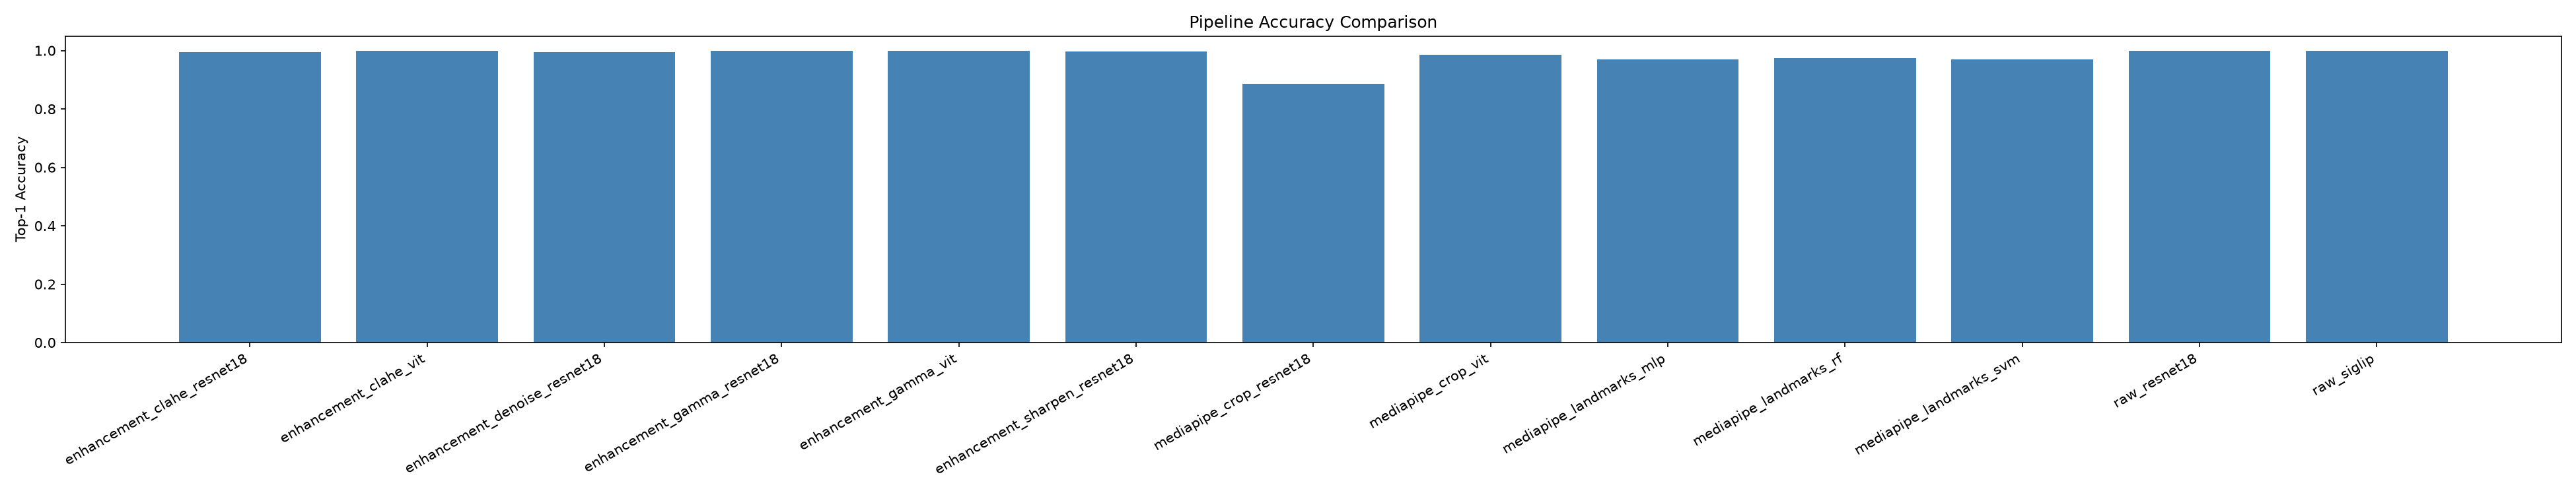
\includegraphics[width=0.85\textwidth]{photos/pipeline_accuracy_comparison.png}
		\end{figure}
	\end{frame}

	\begin{frame}{6.2 Trade-off Latency / FPS}
		\begin{figure}
			\centering
			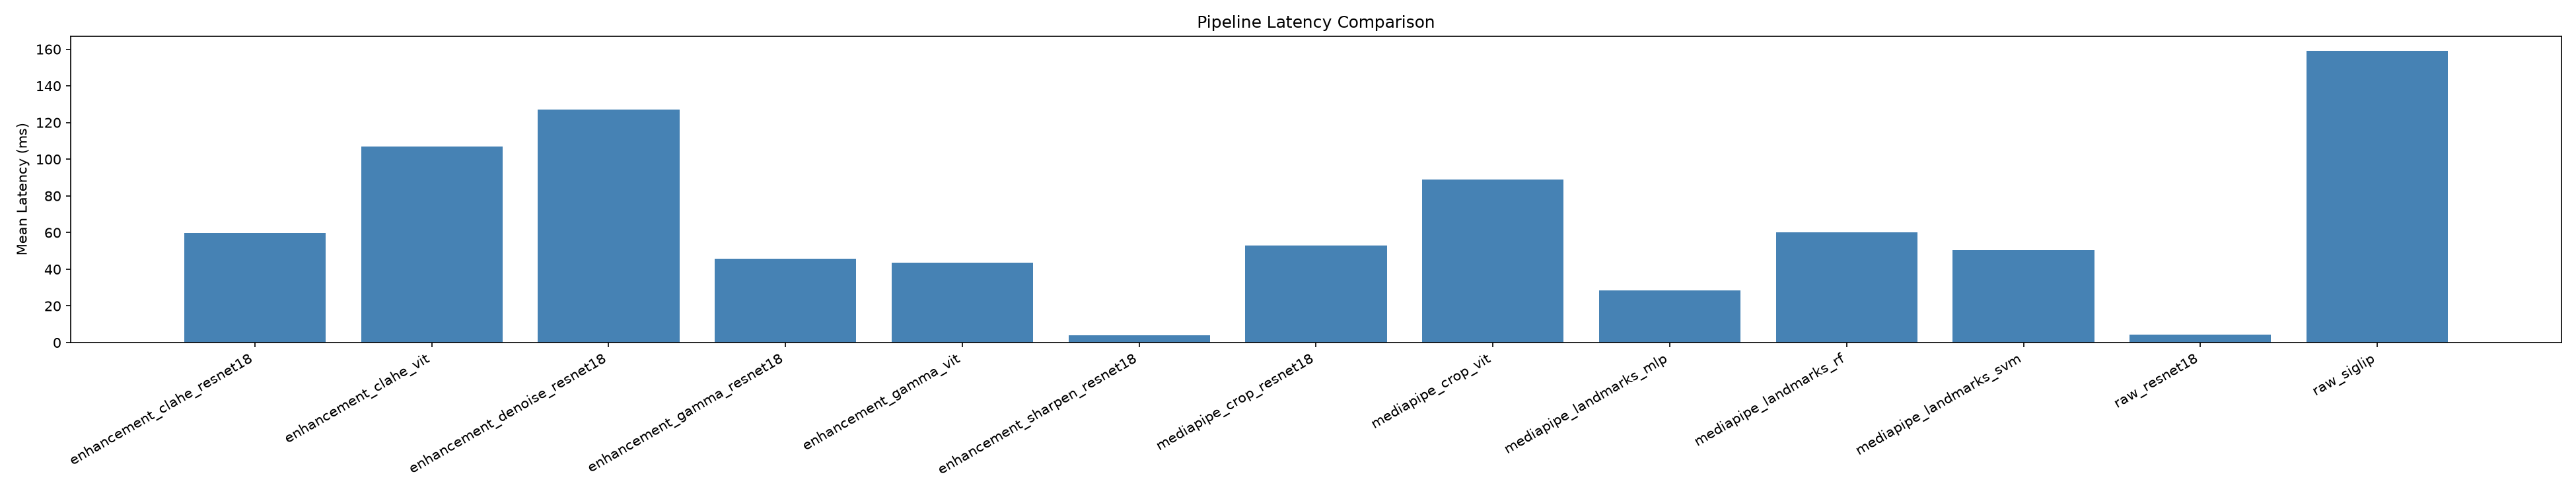
\includegraphics[width=0.8\textwidth]{photos/pipeline_latency_comparison.png}
		\end{figure}
		\footnotesize \textit{Landmark-based (MLP/SVM/RF) và ResNet18 trên ảnh thô có FPS cao nhất, phù hợp ứng dụng thời gian thực.}
	\end{frame}

	\begin{frame}{6.3 Robustness dưới Corruption}
		\begin{figure}
			\centering
			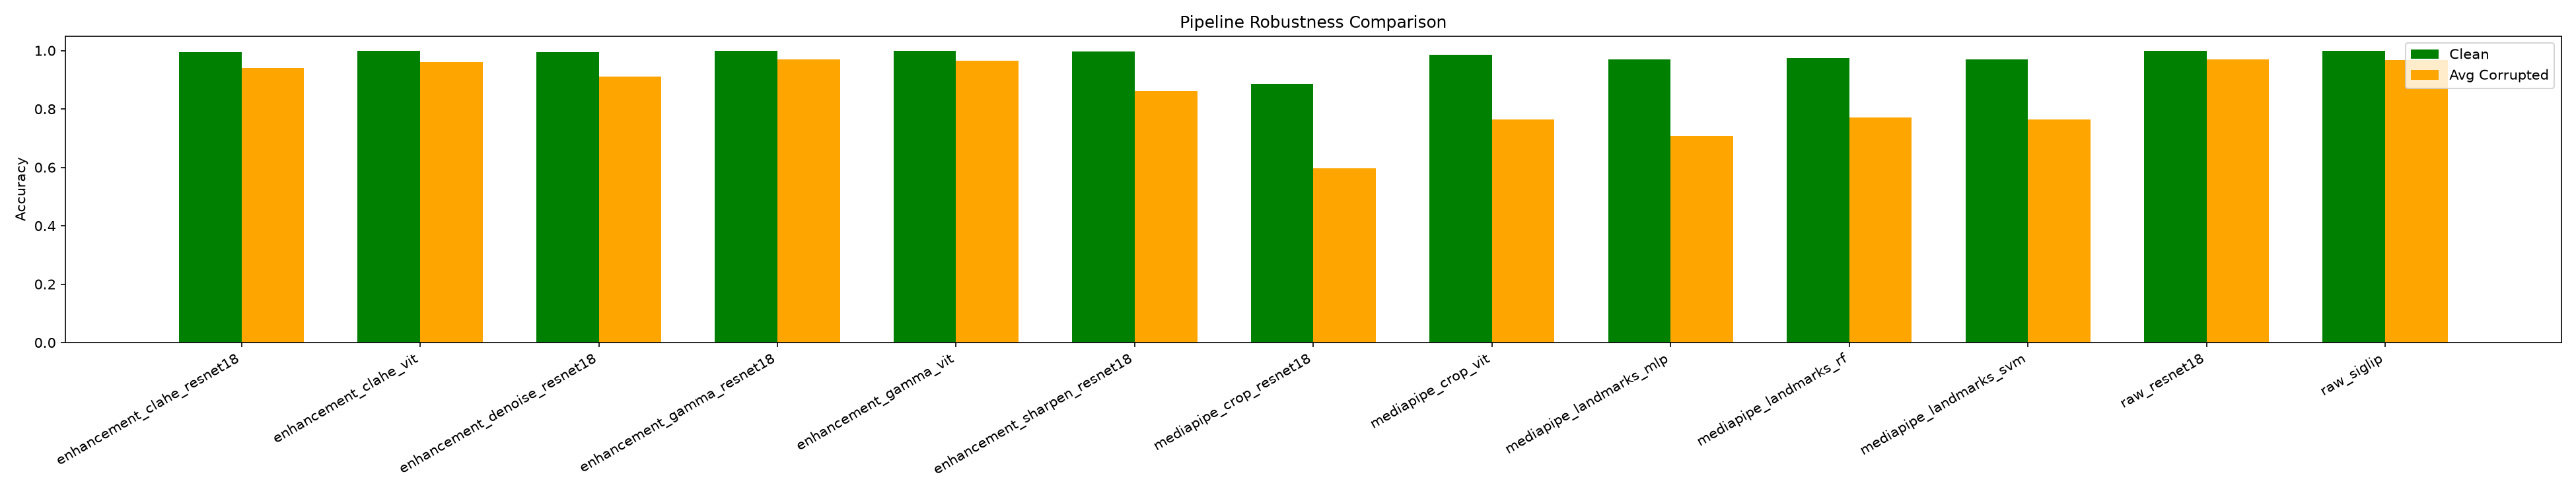
\includegraphics[width=0.85\textwidth]{photos/pipeline_robustness_comparison.png}
		\end{figure}
	\end{frame}

	\begin{frame}{6.4 Qualitative — Module Representation}
		\begin{figure}
			\centering
			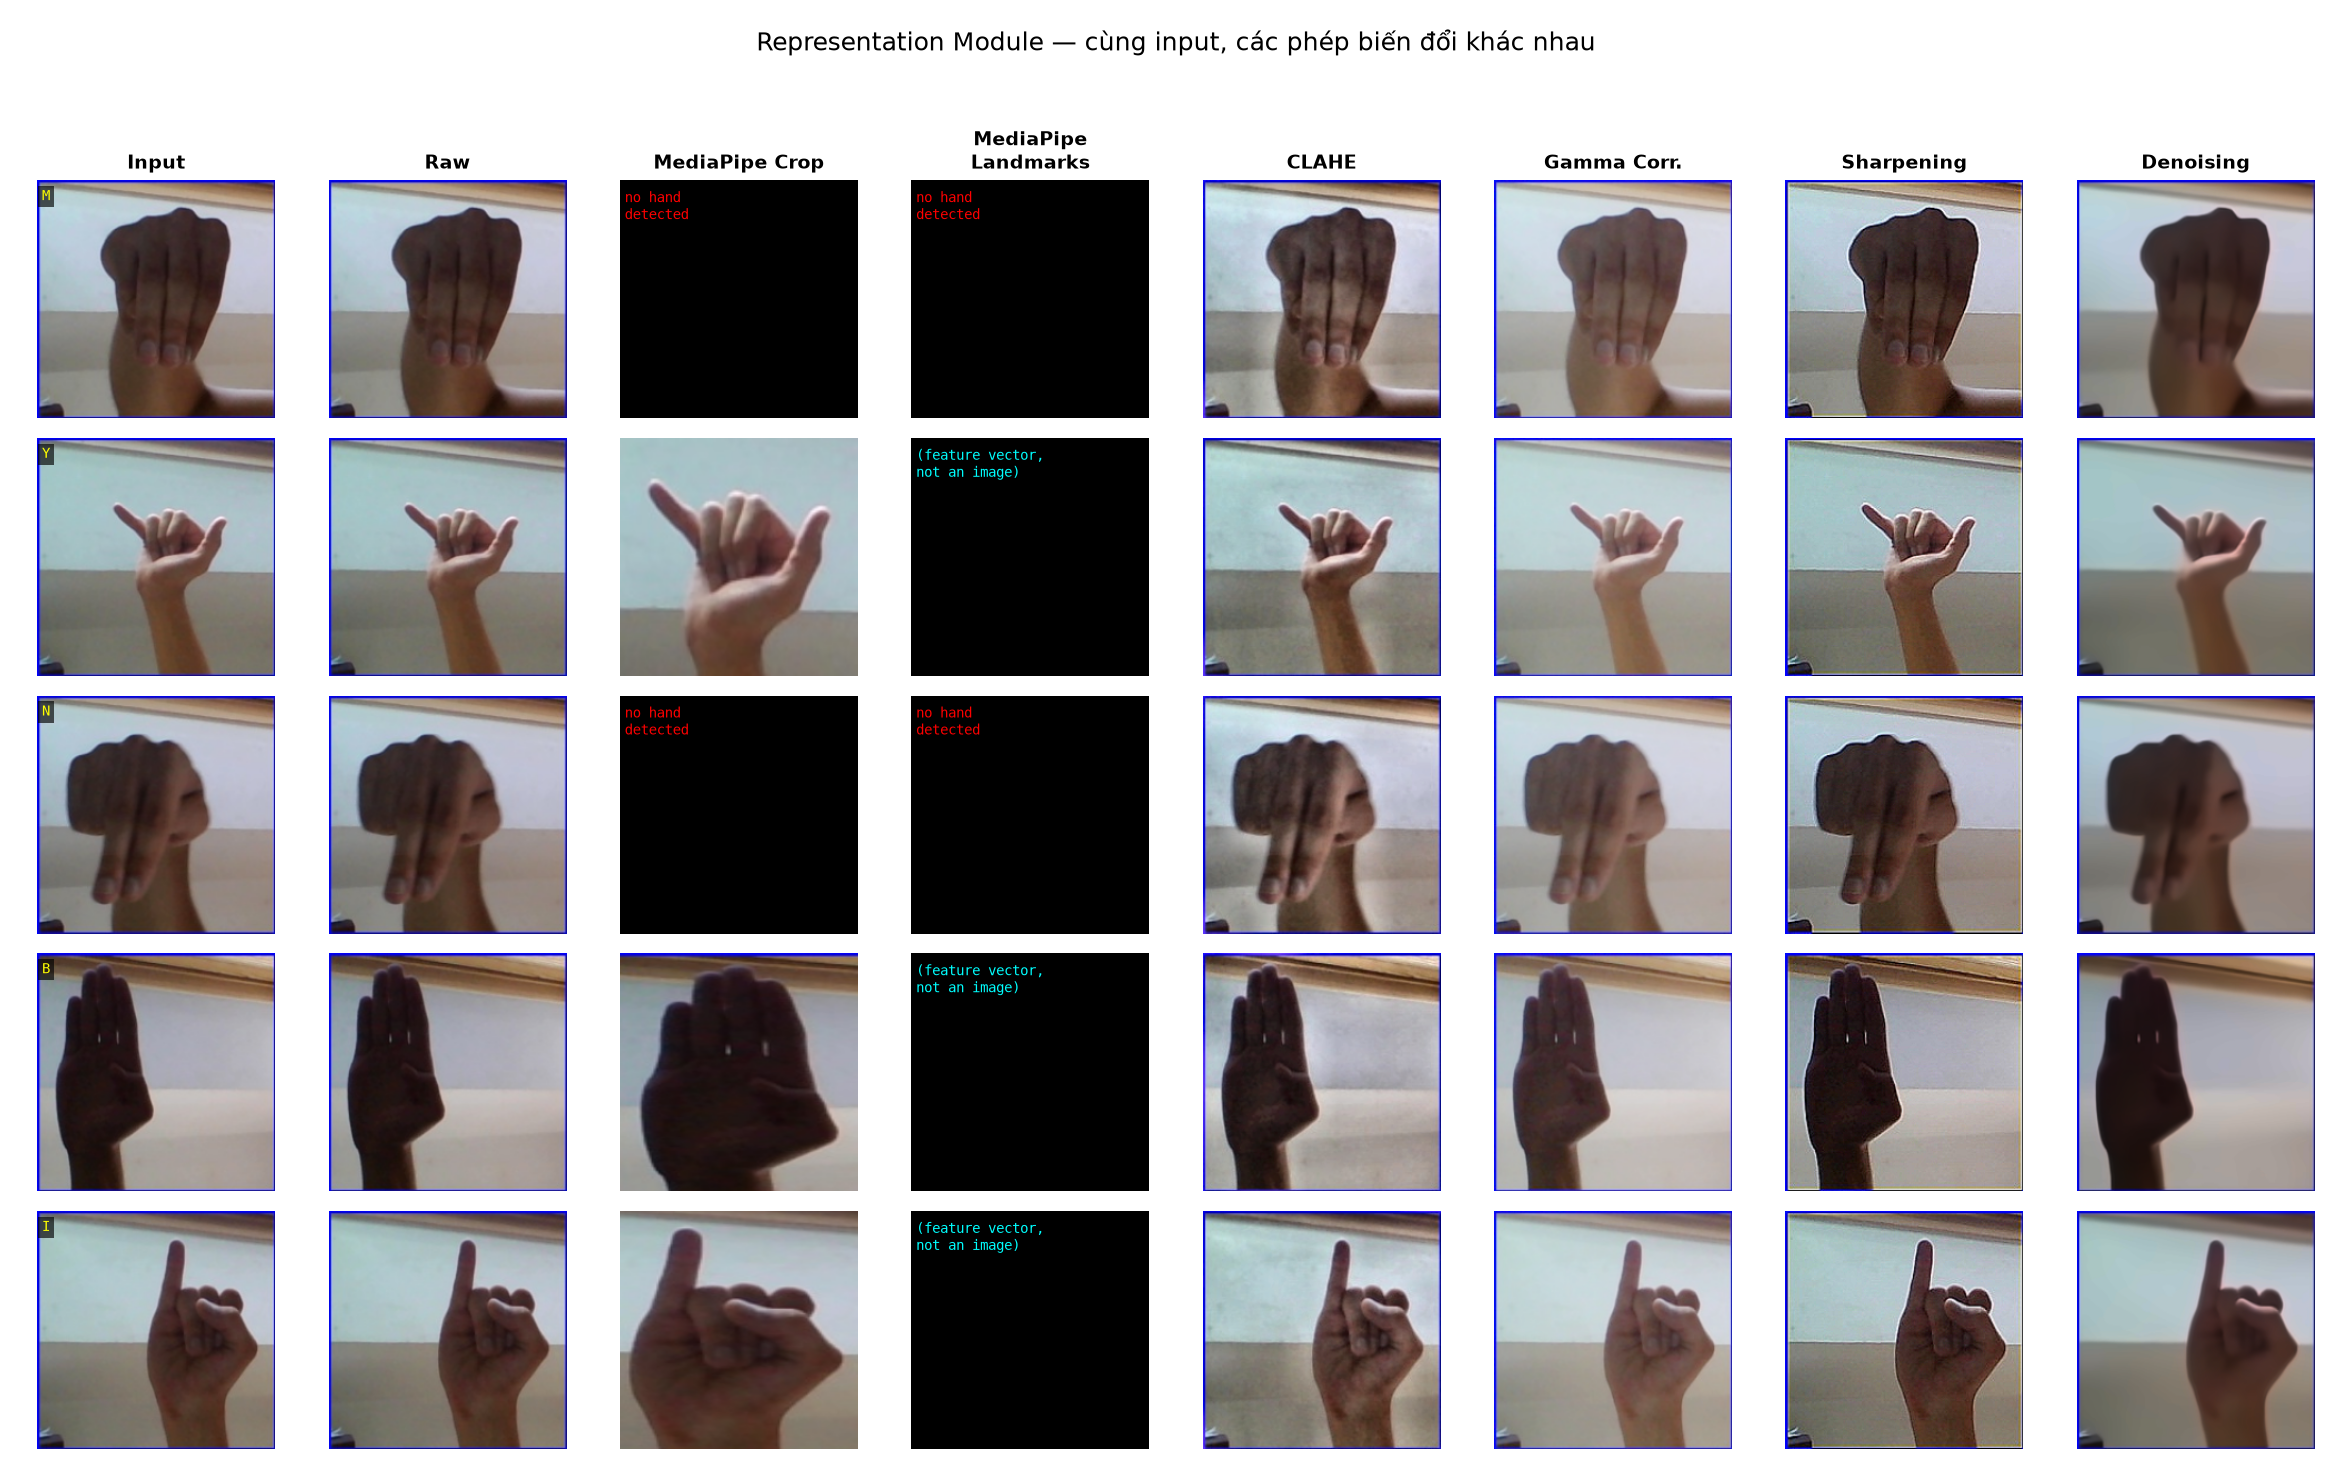
\includegraphics[width=0.95\textwidth]{photos/grid_representation.png}
		\end{figure}
		\footnotesize \textit{Cùng 5 ảnh mẫu, 7 cách biến đổi. Cột MediaPipe (Crop/Landmarks) bị đen ở 3/5 ảnh tối — tay không được phát hiện.}
	\end{frame}

	\begin{frame}{6.5 Qualitative — Module Recognizer (toàn bộ 13 pipeline)}
		\begin{figure}
			\centering
			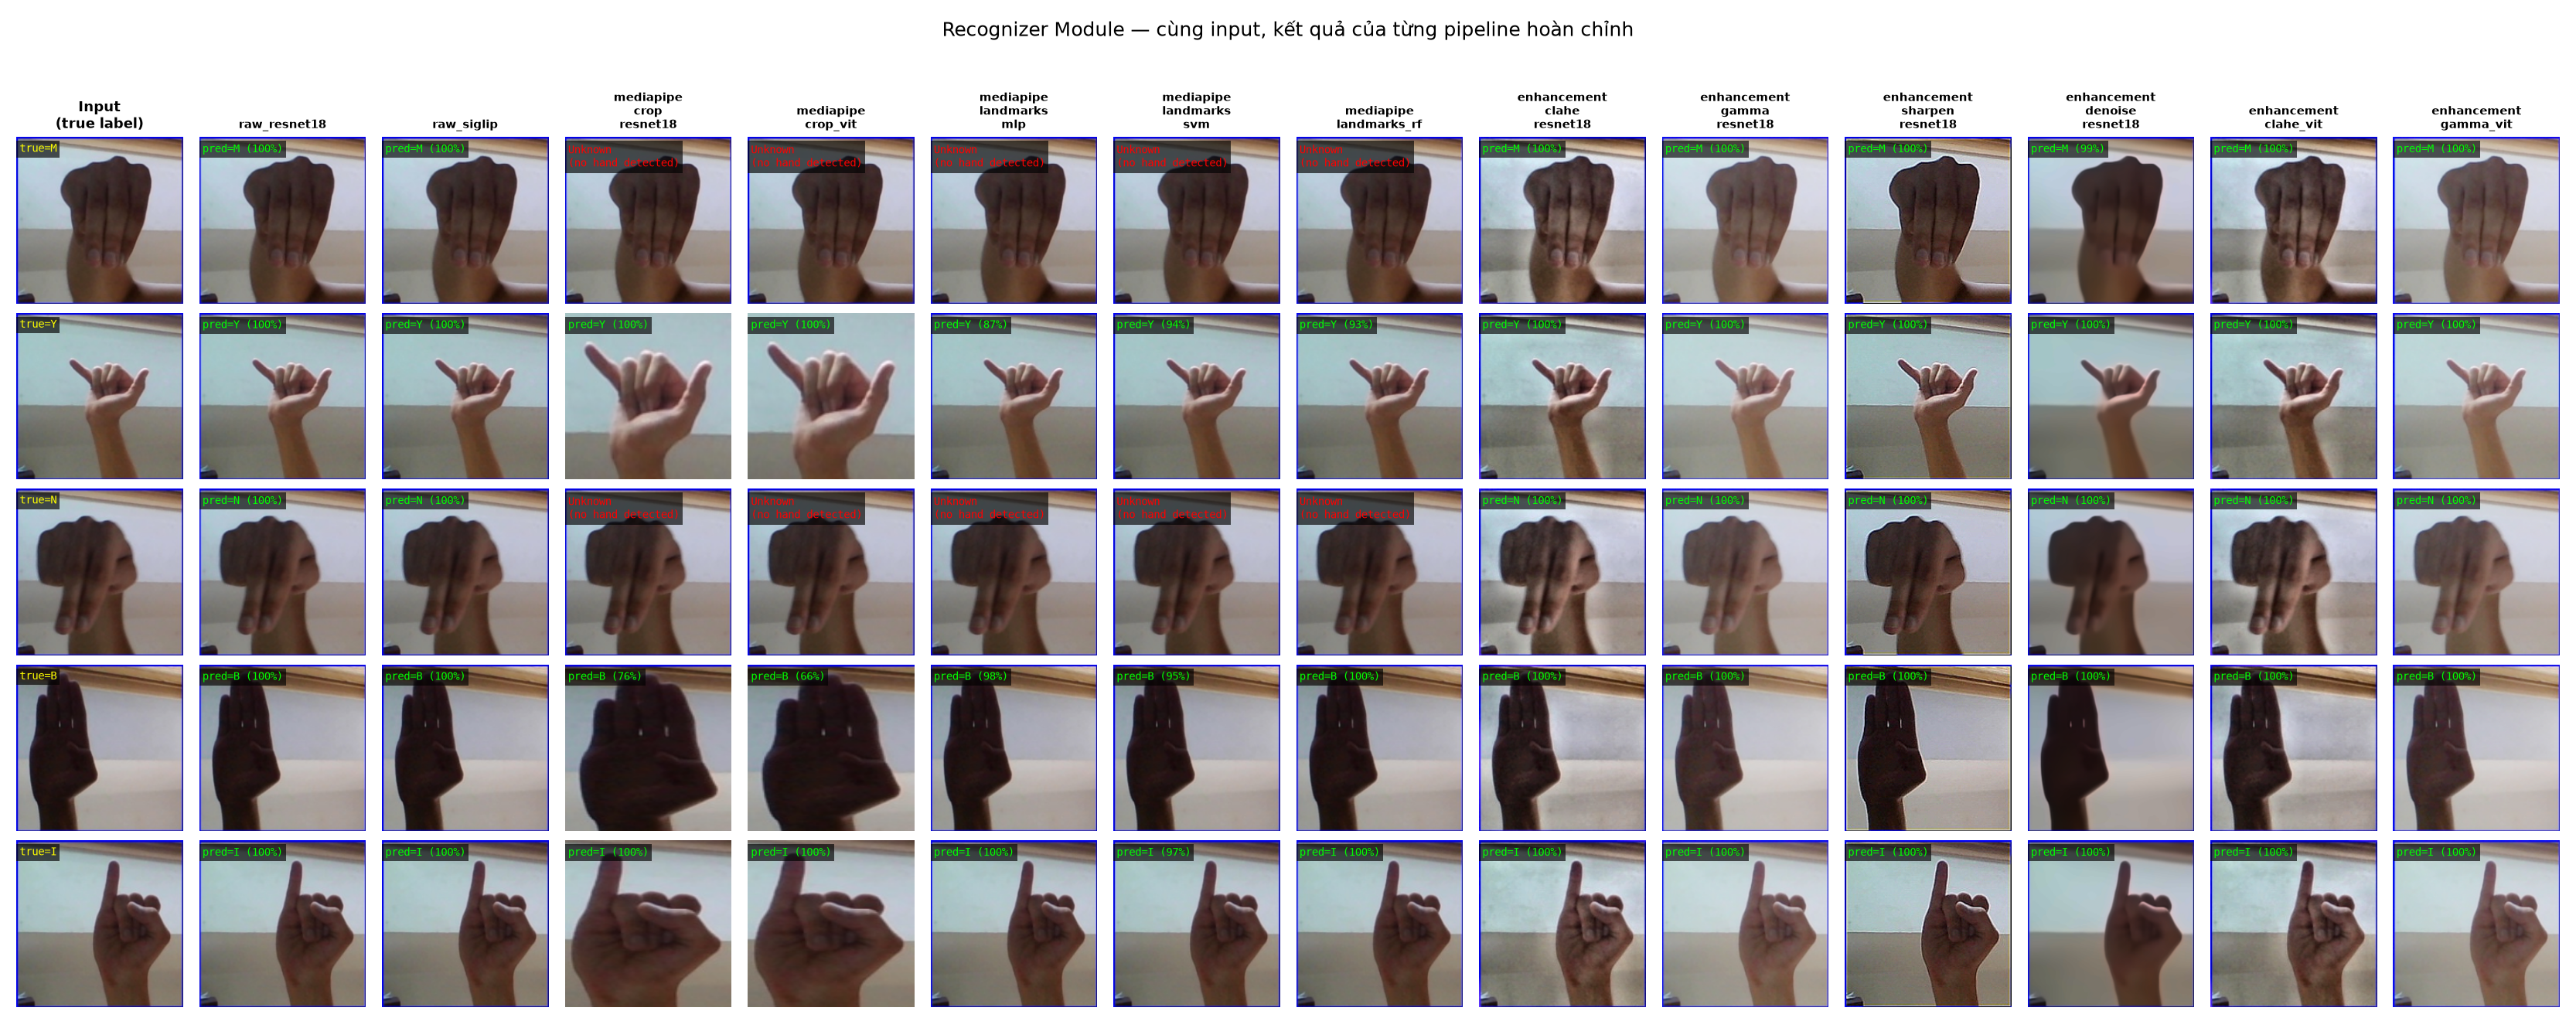
\includegraphics[width=0.97\textwidth]{photos/grid_recognizer.png}
		\end{figure}
		\footnotesize \textit{Overlay xanh = đúng, đỏ = sai. Mọi pipeline dùng MediaPipe đều đỏ giống nhau ở đúng 3 ảnh tối đó — lỗi lan truyền từ representation chung.}
	\end{frame}

	\begin{frame}{6.6 Case Study — "Accuracy cao mà vẫn sập"}
		\begin{columns}[T]
			\begin{column}{0.55\textwidth}
				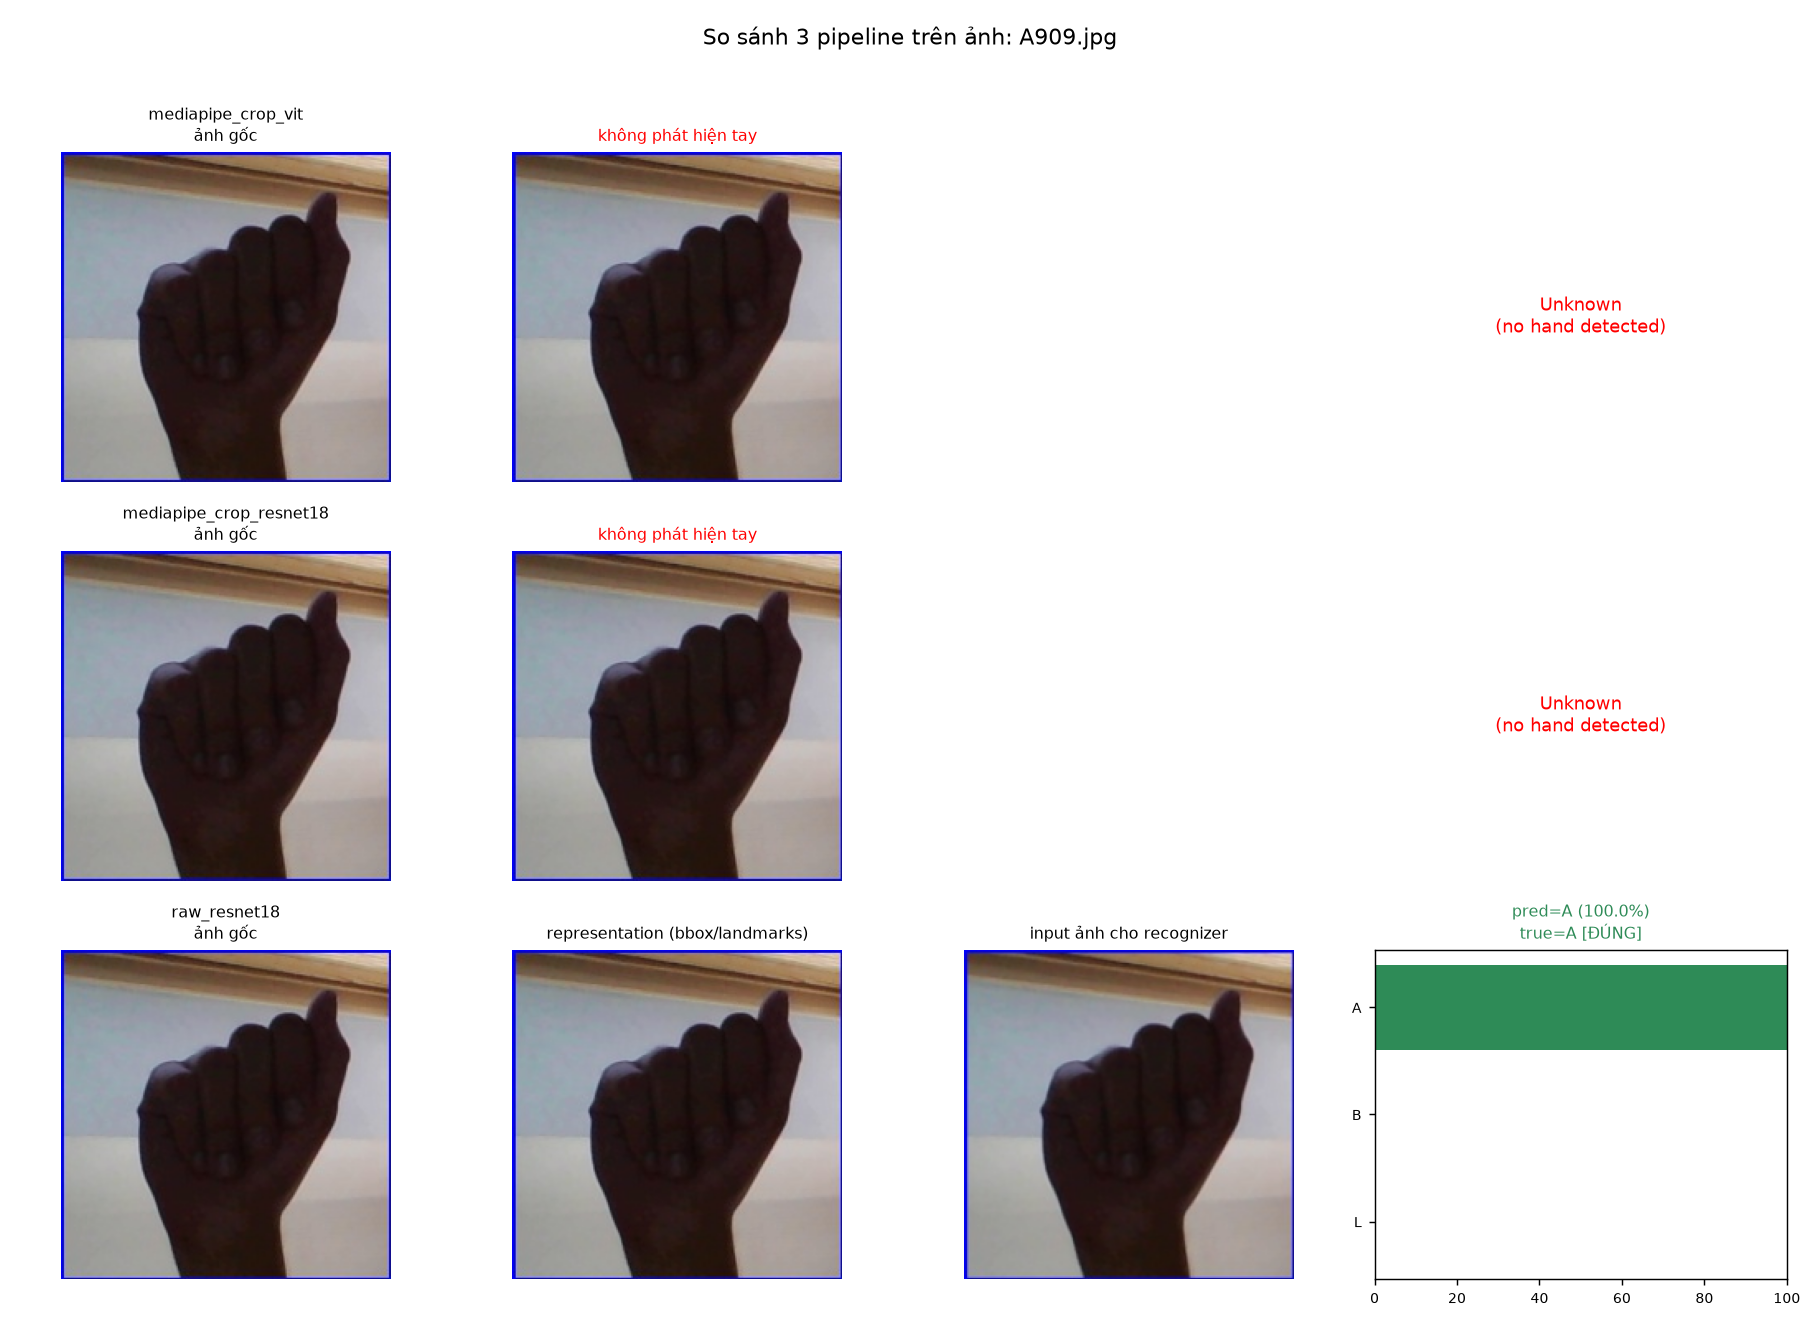
\includegraphics[width=\textwidth]{photos/compare_A909_hand_not_detected.png}
			\end{column}
			\begin{column}{0.43\textwidth}
				\textbf{mediapipe\_crop\_vit}: Clean Acc = 98.5\%

				\vspace{0.5em}
				Nhưng accuracy thực (tính cả Unknown):
				\[
					\frac{2110}{2600} = \alert{\textbf{81.15\%}}
				\]
				\vspace{0.5em}
				\textit{Thấp hơn 17 điểm \% so với số "đẹp" ban đầu — vì 17.15\% ảnh bị MediaPipe bỏ sót tay không được tính vào accuracy chuẩn.}

				\vspace{0.5em}
				\texttt{raw\_resnet18} (không qua bước detect) vẫn nhận đúng "A" 100\% trên đúng ảnh này.
			\end{column}
		\end{columns}
	\end{frame}

	\begin{frame}{6.7 Diễn giải nội bộ CNN — Grad-CAM}
		\begin{columns}[T]
			\begin{column}{0.5\textwidth}
				\centering \footnotesize \texttt{raw\_resnet18}
				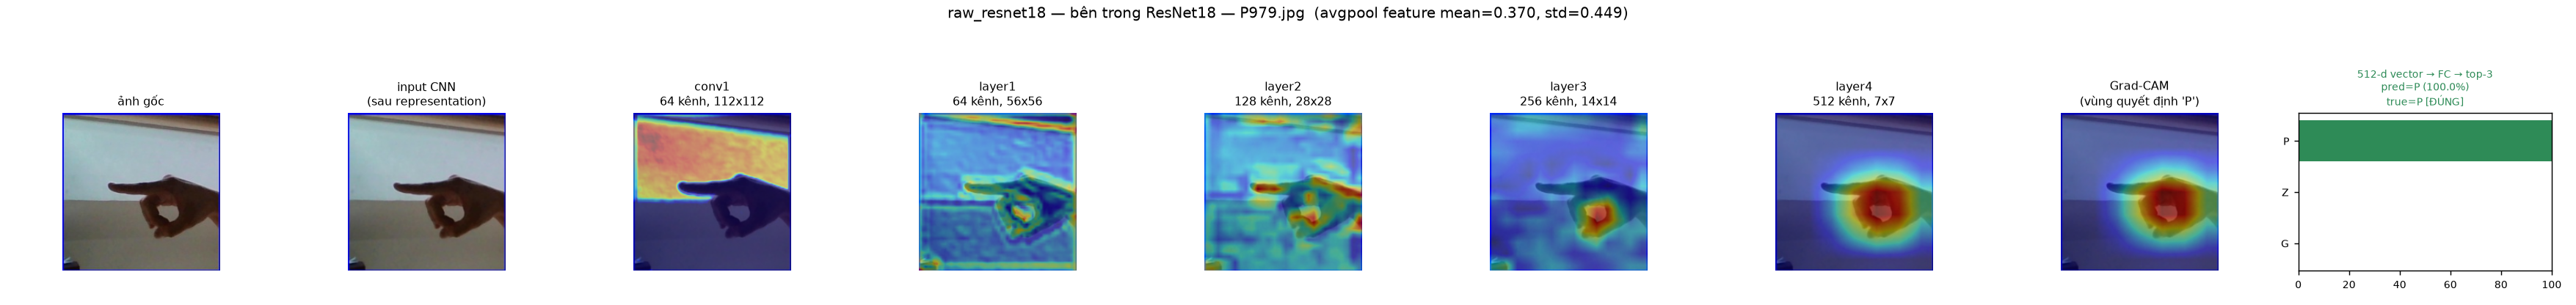
\includegraphics[width=\textwidth]{photos/cnn_internals_raw_resnet18_P979.png}
			\end{column}
			\begin{column}{0.5\textwidth}
				\centering \footnotesize \texttt{mediapipe\_crop\_resnet18}
				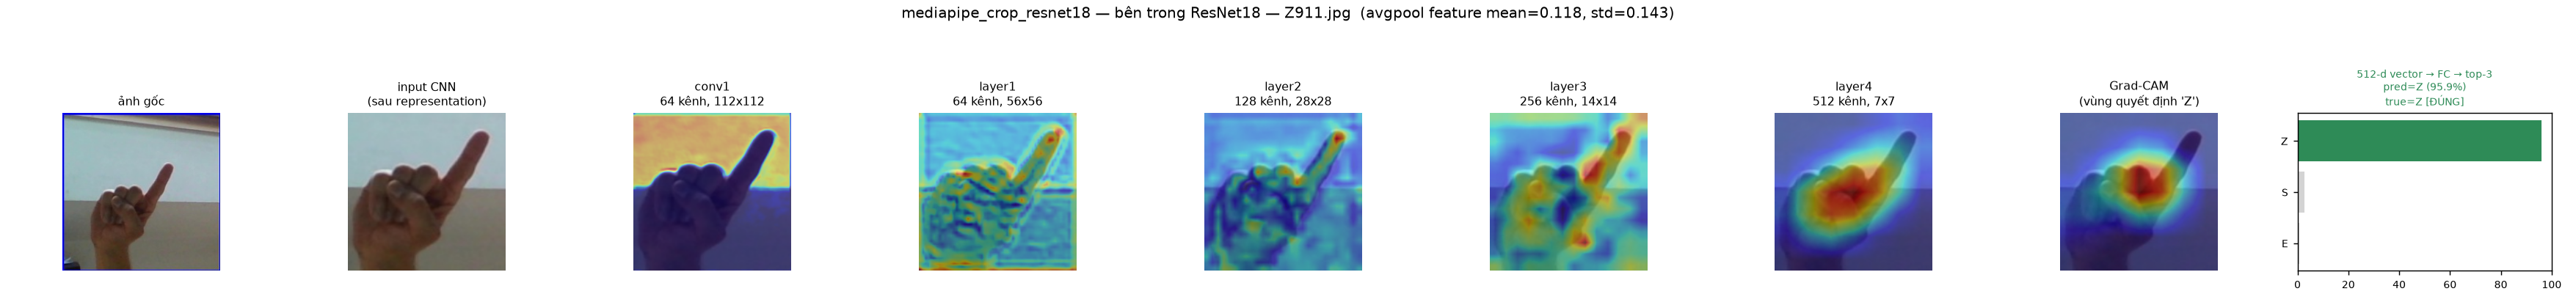
\includegraphics[width=\textwidth]{photos/cnn_internals_mediapipe_crop_resnet18_Z911.png}
			\end{column}
		\end{columns}
		\footnotesize \textit{Activation map co dần qua conv1$\to$layer4 (224$\to$7), kênh tăng 64$\to$512. Grad-CAM khoanh đúng vùng bàn tay quyết định nhãn dự đoán.}
	\end{frame}

	\begin{frame}{6.8 Không gian đặc trưng — UMAP / t-SNE theo lớp}
		\begin{figure}
			\centering
			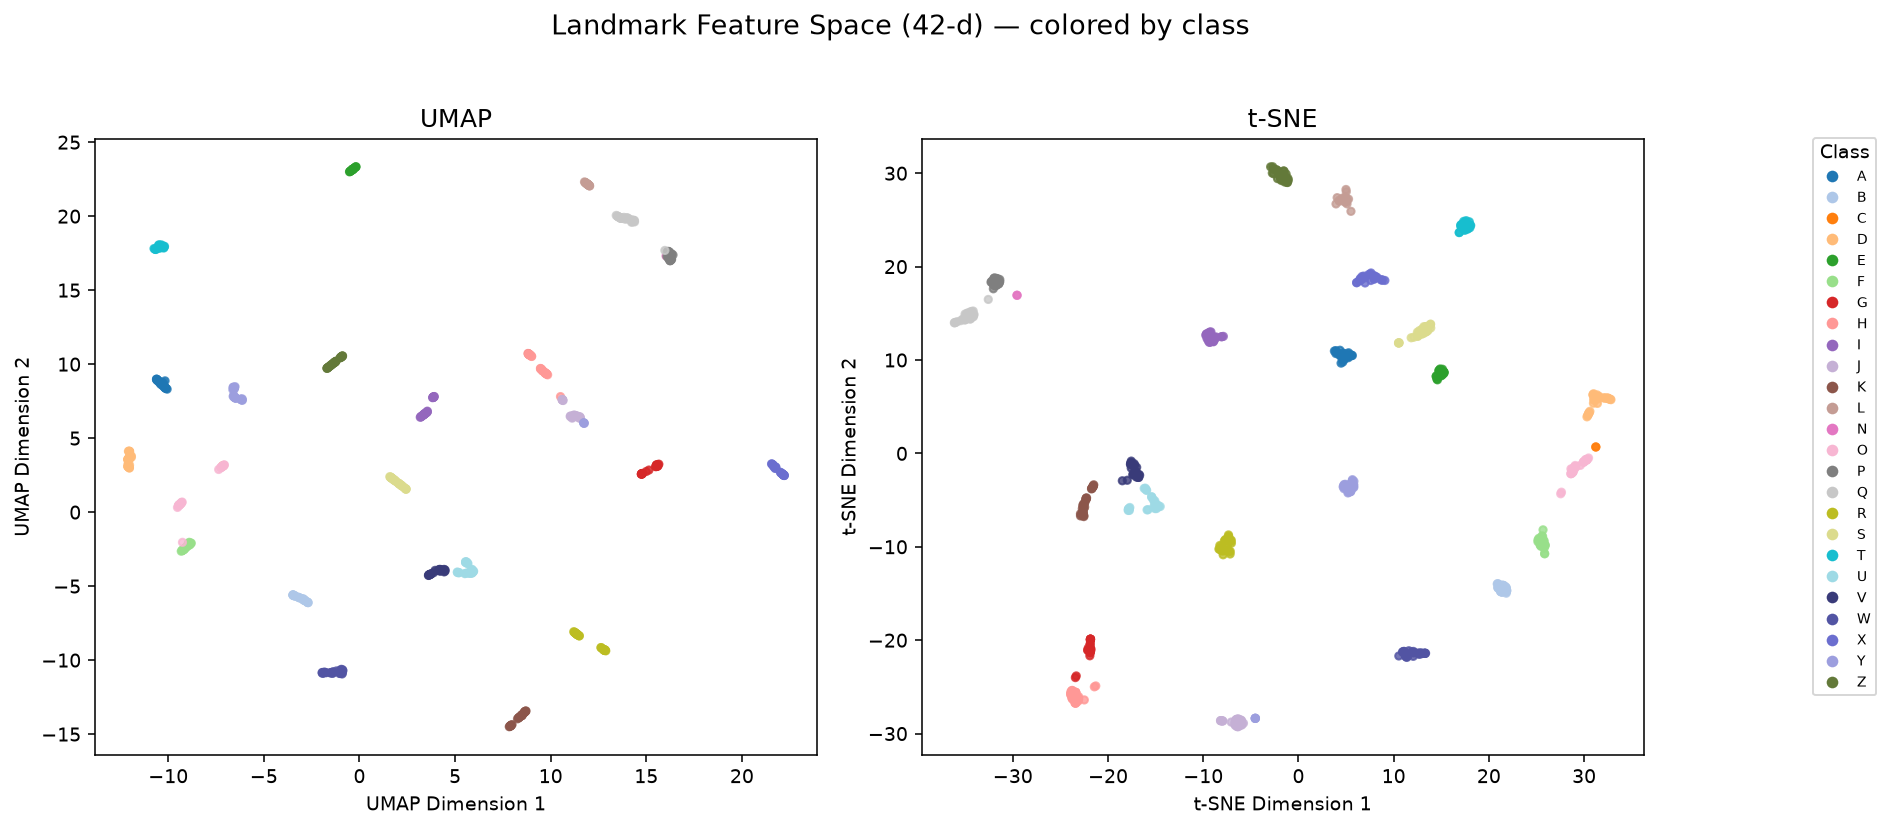
\includegraphics[width=0.85\textwidth]{photos/embedding_landmarks_by_class.png}
		\end{figure}
		\footnotesize \textit{Vector landmark 42-d, lấy mẫu 30 ảnh/lớp trên test\_split. 26 lớp A--Z tách cụm rõ ràng — landmark là đặc trưng phân biệt tốt cho MLP/SVM/RF.}
	\end{frame}

	\begin{frame}{6.9 Không gian đặc trưng — Representation có làm lệch không?}
		\begin{figure}
			\centering
			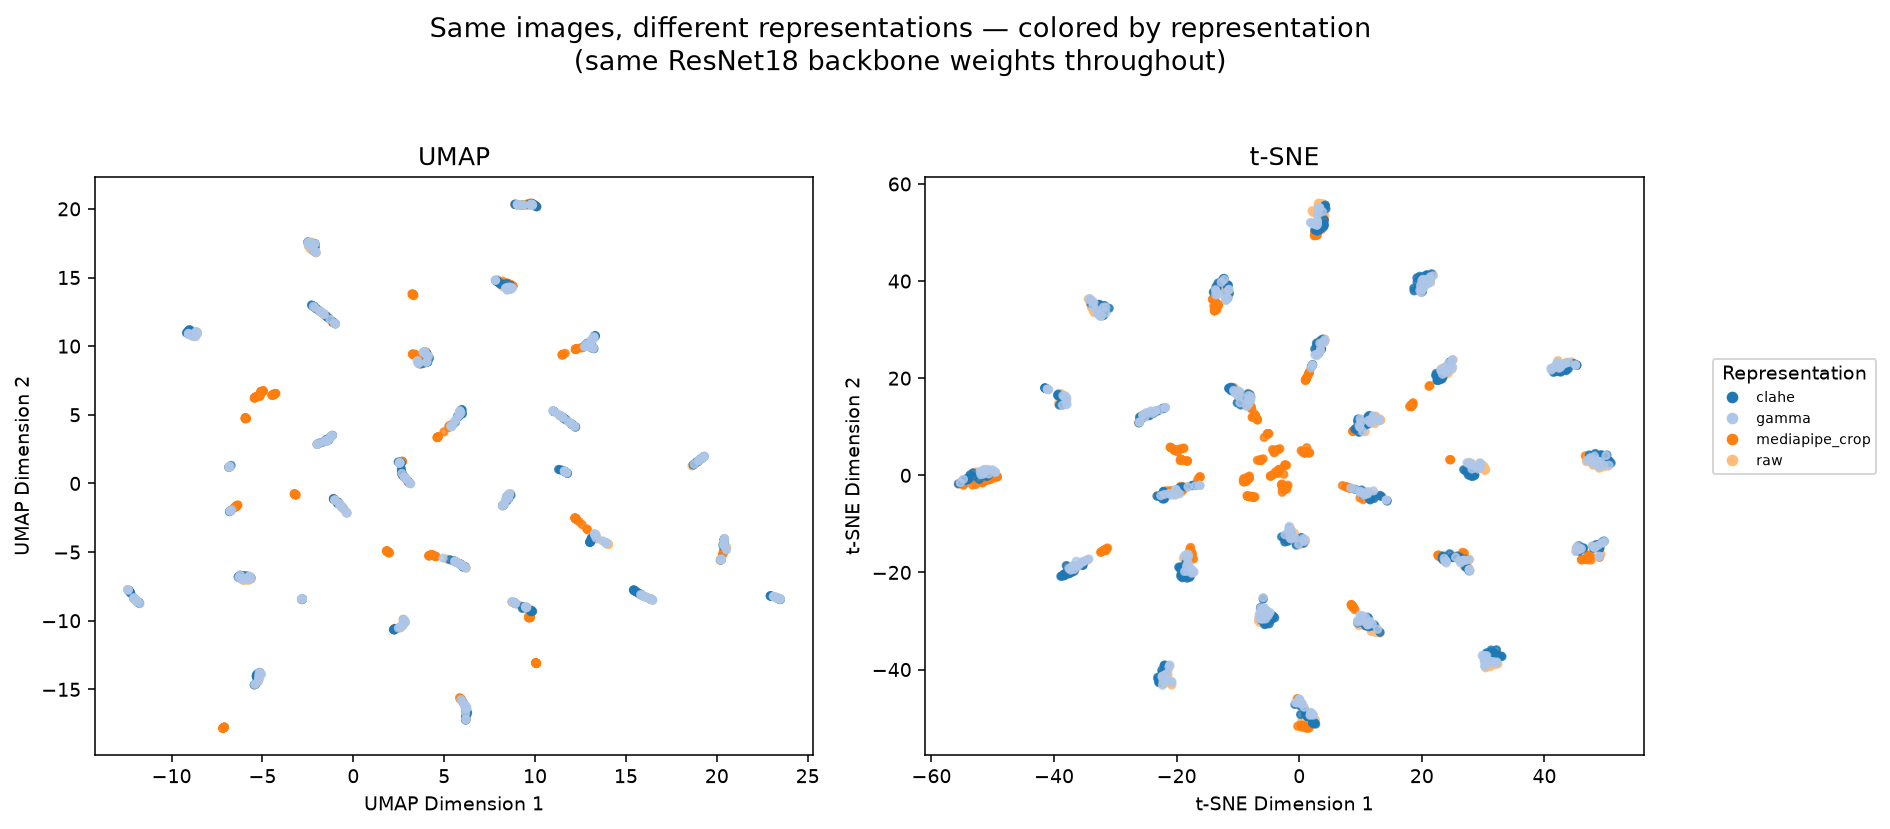
\includegraphics[width=0.78\textwidth]{photos/embedding_representation_shift.png}
		\end{figure}
		\footnotesize \textit{Cùng ảnh, 4 representation khác nhau, cùng backbone ResNet18. CLAHE/Gamma/Raw nằm rất gần nhau (cùng cụm nhỏ) — enhancement nhẹ không đổi nhiều không gian đặc trưng. MediaPipe Crop (cam) tách hẳn vị trí khác — đổi representation mới thực sự dịch chuyển không gian đặc trưng.}
	\end{frame}

	% =================================================================
	\section{Kết luận}
	% =================================================================
	\begin{frame}{7. Kết luận}
		\begin{columns}[T]
			\begin{column}{0.32\textwidth}
				\begin{block}{\small Đánh giá đúng metric}
					\footnotesize Clean accuracy "chuẩn" có thể che giấu thất bại thực — phải dùng accuracy tính cả Unknown.
				\end{block}
			\end{column}
			\begin{column}{0.32\textwidth}
				\begin{block}{\small Lỗi 2 tầng nguy hiểm hơn lỗi 1 tầng}
					\footnotesize Thêm bước detect tay (MediaPipe) thêm 1 điểm gãy — robustness sập về 0\% dù backbone mạnh.
				\end{block}
			\end{column}
			\begin{column}{0.32\textwidth}
				\begin{block}{\small Đơn giản có thể bền hơn}
					\footnotesize raw/enhancement + ResNet18/ViT không bao giờ sập dưới 70\% ở corruption xấu nhất.
				\end{block}
			\end{column}
		\end{columns}

		\vspace{1em}
		\begin{alertblock}{Limitations}
			\footnotesize Một số representation chưa hoàn thiện (YOLO-crop, segmentation-mask, fusion là stub); chỉ 1 dataset (ASL Alphabet, ảnh studio).
		\end{alertblock}

		\begin{block}{Future Work}
			\footnotesize Hoàn thiện YOLO-crop/segmentation/fusion; đánh giá trên dữ liệu webcam thực tế ngoài studio; thử fallback raw khi MediaPipe gãy.
		\end{block}
	\end{frame}

	% =================================================================
	\section{Phân công công việc}
	% =================================================================
	\begin{frame}{Work Assignment}
		\small
		\begin{table}
			\centering
			\begin{tabular}{p{0.3\textwidth}p{0.6\textwidth}}
				\toprule
				\textbf{Thành viên} & \textbf{Nhiệm vụ} \\
				\midrule
				Trần Quang Hưng - 20235502 & YOLOv8 pipeline, chuẩn bị dataset, hand detection \\
				\addlinespace
				Đỗ Đăng Vũ - 20235578 & Classifier (ResNet/MobileNet) \& transforms, đánh giá robustness, visualization \\
				\addlinespace
				Lê Hoàng Tùng - 20235572 & Demo (OpenCV/Gradio), evaluation pipeline, báo cáo \\
				\bottomrule
			\end{tabular}
		\end{table}
	\end{frame}

	% =================================================================
	\hustcontactpage{\hfill THÔNG TIN LIÊN HỆ \hfill }{
		\textbf{Nhóm:} Computer Vision Capstone — HUST \\
		\vspace{0.5cm}
		\begin{itemize}
			\item \textbf{Github:} \url{https://github.com/}
		\end{itemize}
		\vspace{1cm}
		\textit{Xin chân thành cảm ơn Hội đồng đã lắng nghe!}
	}

	% =================================================================
	\useStyleLogoOnly
	\setbeamertemplate{bibliography item}[text]

	\begin{frame}[allowframebreaks]{Tài liệu tham khảo}
		\begin{thebibliography}{99}
			\bibitem{mediapipe}
			C. Lugaresi et al., ``MediaPipe: A Framework for Building Perception Pipelines,'' arXiv:1906.08172, 2019.

			\bibitem{resnet}
			K. He, X. Zhang, S. Ren, J. Sun, ``Deep Residual Learning for Image Recognition,'' CVPR, 2016.

			\bibitem{siglip}
			X. Zhai et al., ``Sigmoid Loss for Language Image Pre-Training (SigLIP),'' ICCV, 2023.

			\bibitem{aslalphabet}
			Kaggle, ``ASL Alphabet Dataset,'' \url{https://www.kaggle.com/datasets/grassknoted/asl-alphabet}.

			\bibitem{umap}
			L. McInnes, J. Healy, J. Melville, ``UMAP: Uniform Manifold Approximation and Projection,'' arXiv:1802.03426, 2018.

			\bibitem{tsne}
			L. van der Maaten, G. Hinton, ``Visualizing Data using t-SNE,'' JMLR, 2008.

			\bibitem{gradcam}
			R. Selvaraju et al., ``Grad-CAM: Visual Explanations from Deep Networks via Gradient-based Localization,'' ICCV, 2017.
		\end{thebibliography}
	\end{frame}

	\hustthankyou

\end{document}
